% !TEX root = morphkasten.tex

\section{Containererkennung (detailliert)}


%##############
\subsection{Sensor}

Grafik

\begin{table}[h]
\begin{tabular}{p{0.5\textwidth} | p{0.5\textwidth}}


 \textbf{Vorteile} & \textbf{Nachteile} \\ \hline
	 
\begin{itemize}
\item Vorteil 1
\item Vorteil 2
\item Vorteil 3
\item ...
\end{itemize}

 
 &
 
\begin{itemize}
\item Nachteil 1
\item Nachteil 2
\item Nachteil 3
\item ...
\end{itemize}

\end{tabular}
\end{table}

\begin{table}[h]
\begin{tabular}{p{0.5\textwidth}p{0.5\textwidth}}


 \textbf{Risiken} & \\ \hline
	 
\begin{itemize}
\item Risiko 1
\item Risiko 2
\end{itemize}
&
\begin{itemize}
\item Risiko 3
\item ...
\end{itemize}

 
\end{tabular}
\end{table}

\pagebreak


%##############
\subsection{Bilderkennung}
\begin{figure}[h!]%Position festigen
\centering
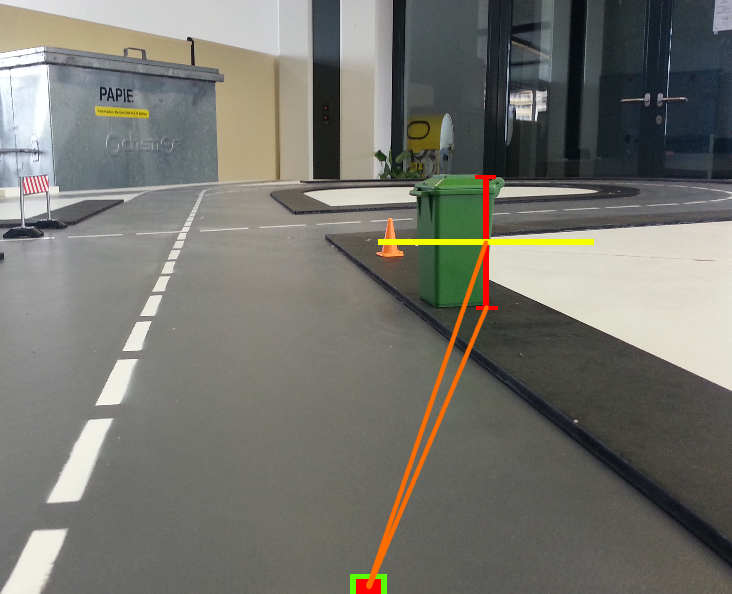
\includegraphics[width=0.7\textwidth]{fig/containererkennung_detailliert_bilderkennung.png}
\caption{Bilderkennung Container}
\label{fig:Bilderkennung Container}
\end{figure}
\begin{table}[h]
\begin{tabular}{p{0.5\textwidth} | p{0.5\textwidth}}


 \textbf{Vorteile} & \textbf{Nachteile} \\ \hline
	 
\begin{itemize}
\item keine Sensoren zur Seite benötigt
\end{itemize}

 
 &
 
\begin{itemize}
\item Berechnung des Abstands muss auf wenige Milimeter stimmen
\item Keine Korrektur mehr möglich, wenn der Container aus dem Kamerbereich verschwindet
\end{itemize}

\end{tabular}
\end{table}

\begin{table}[h]
\begin{tabular}{p{0.5\textwidth}p{0.5\textwidth}}


 \textbf{Risiken} & \\ \hline
	 
\begin{itemize}
\item Ungenauigkeit bei der Distanzabschätzung
\item Container kann zum Teil von anderen Gegeständen verdeckt sein
\end{itemize}

 
\end{tabular}
\end{table}

\pagebreak
